\documentclass[11pt,a4paper]{article}
\usepackage[margin=25mm]{geometry}
\usepackage{booktabs,hyperref,graphicx}
\setlength{\parindent}{0pt}\setlength{\parskip}{6pt}
\begin{document}
{\small MASTER'S THESIS EXPERIMENT REPORT \hfill 13 November 2026}

{\LARGE\bfseries Conditional DiffTraj on Porto taxis and Turin buses\par}
Jingting Liu

\section*{Question and data}
Given the attributes of a long taxi journey, how closely do trajectories sampled by DiffTraj reproduce the lengths and spatial distribution of observed journeys? Zhu et al. studied taxi GPS trajectories from Chengdu and Xi'an in their main experiment and reported an additional Porto comparison in Appendix C, Table 5, where DiffTraj was compared with VAE, TrajGAN, DiffWave and Diff-LSTM on four distributional measures. The Porto experiment reproduces the published benchmark under a documented long-trip rule. A second experiment applies the same generator to observed Turin bus journeys.

The UCI Porto taxi trajectory corpus (source linked below) records taxi positions at 15-second intervals. Each row describes a journey with a taxi identifier, departure timestamp and ordered longitude--latitude polyline. From 1,710,670 rows, we retained complete, finite tracks containing at least 120 original positions before interpolation. At the native cadence, 120 positions span 29 min 45 s. The resulting 55,267 journeys from 439 taxis represent the long-trip population. The paper describes a 120-point rule in Appendix B.1, but gives no separate retained count or exact split for Porto.

We partitioned by taxi identity to keep vehicles disjoint. The training partition contained 46,470 journeys, the development partition 5,241 and the reserved partition 3,556. We used 512 fixed development requests for checkpoint selection and sampled 3,000 reserved journeys for the final comparison.

\section*{Model and training}
DiffTraj represents each journey as two coordinate channels interpolated to 200 positions. During training, Gaussian noise is added to an observed trajectory. A temporal U-Net takes the noisy coordinates, the noise level and a trip header and predicts the injected noise by minimizing mean squared error. The header specifies departure-time bin, distance, duration, original point count, average displacement, average speed, and origin and destination cells. Sampling begins with Gaussian noise and iteratively denoises it. We restore the original sample count before scoring. Supplying distance and endpoints makes this an evaluation of conditional generation.

We trained the released coordinate architecture from scratch for 200 epochs with 500 noise levels, 100 reverse sampling steps and global batch size 1,024 on four NVIDIA L20 GPUs (256 journeys per GPU). Inputs were normalized from training data. The authors' published training loop uses fixed-rate AdamW and saves ordinary network weights every ten epochs. Following instability in an earlier local fit, the two runs reported here used AdamW, gradient clipping at norm 1 and cosine learning-rate decay from 0.0002 to 0.00002. Epochs 193 and 179 minimized fixed development noise loss for seeds 42 and 43, respectively. The second fit changed initialization, training order and training noise while retaining the data, validation rule, sampling noise and evaluation requests.

\newpage
\section*{Results against the published Porto benchmark}
Density and OD errors compare point occupancy and ordered origin--destination cell frequencies on a $16\times16$ grid. Length error compares distributions of cumulative journey distance. All three use Jensen--Shannon divergence (JS), with zero for identical distributions. Our length histogram uses 20 training-quantile bins. Our pattern F1 measures the overlap of the 20 most frequently visited cells.

\begin{center}
\begin{tabular}{lrrrr}\toprule
 & Density JS $\downarrow$ & OD JS $\downarrow$ & Length JS $\downarrow$ & Pattern F1 $\uparrow$\\\midrule
Published Table 5 & .00870 & .01320 & .02420 & .847\\
Long trips, seed 42 & .01357 & .00594 & .00635 & .750\\
Long trips, seed 43 & .00944 & .00698 & .00395 & .800\\
\bottomrule\end{tabular}
\end{center}

\textbf{How the grid changes hotspot F1.} We scored each set of 3,000 draws against identical observed journeys under three grid definitions. Each grid divides the specified longitude and latitude ranges into 16 equal intervals per axis. We count GPS points in each cell and rank the cells separately for observed and generated trips. Both hotspot sets contain 20 cells, so F1 equals the number of shared cells divided by 20.

\begin{center}\small
\begin{tabular}{lrr}\toprule
Training coordinates used to set grid edges & Seed 42: hits / F1 & Seed 43: hits / F1\\\midrule
Long trips, full min--max (primary) & 15/20: 0.750 & 16/20: 0.800\\
All eligible lengths sampled for training, full min--max & 17/20: \textbf{0.850} & 16/20: 0.800\\
Same sample, 1st--99th percentile per axis & 15/20: 0.750 & 16/20: 0.800\\\bottomrule
\end{tabular}\end{center}
For seed 42 the shared full-range grid places two additional cells in the overlap. Seed 43 has 16 overlapping cells on every grid. Only the scoring boundaries change; all three rows evaluate the long-trip model. Full-range grids clip outlying points to the edge; the percentile grid excludes overflow from hotspot ranking. The shared-grid score is close to the published 0.847, whose Porto boundaries and hotspot count remain unspecified.

\textbf{What does the length score mean in kilometres?} The observed median was 13.96 km, compared with 12.39 and 12.64 km for seeds 42 and 43. Across requests, generated length averaged 2.01 and 1.51 km below observed length. The first Wasserstein distance between the distributions was 2.28 and 1.92 km, respectively: this measures the average separation of corresponding length quantiles. A small binned JS therefore coexists with a measurable shortfall in distance.

\textbf{Conclusion.} We reproduced the conditional training and sampling procedure on public Porto GPS data under an explicit long-trip rule. Both fits generated shorter median trips and recovered 15 to 17 of the 20 observed hotspots across the specified grids. The scope of this result is journeys of at least 120 recorded positions. 

\newpage
\section*{Turin buses: data, training and evaluation}
The GTT vehicle-position feed supplied 354,114 distinct GPS fixes in a 24-hour collection covering the 12 November service day. Matching vehicle positions to the official timetable and fleet catalogue yielded 3,262 bus journey candidates with terminal coverage. Both ends had to lie within 200 m of the scheduled terminals, observed endpoint times within 15 minutes of schedule, and observed duration at least 70\% of scheduled duration. The median bus journey contains 46 positions. The median interval across retained bus and tram segments was 63 s. A 120-point cutoff would remove every eligible bus journey.

Splitting by vehicle gave 2,555 training, 366 development and 341 reserved journeys. Both fits used the Porto network and eight trip attributes, measured elapsed duration and local departure time. Only buses entered the experiment; no vehicle-class input was supplied. At global batch 1,024, 200 epochs on Turin data give 600 optimizer updates. Reducing the batch to 56 gives 9,200 updates, matching the Porto count. The smaller batch also changes gradient variability. The two training seeds used identical evaluation requests and sampling noise.

\begin{center}\small
\begin{tabular}{lrrrr}\toprule
Turin, 341 reserved requests & Density JS & OD JS & Length JS & Hotspot F1\\\midrule
Batch 1,024, seed 42 & .0607 & .6513 & .1387 & .85\\
Batch 1,024, seed 43 & .4931 & .6889 & .3718 & .15\\
Batch 56, seed 42 & .0120 & .3187 & .0515 & .95\\
Batch 56, seed 43 & .0171 & .3375 & .0611 & .95\\
Observed development vs. reserved & .0587 & .3136 & .0895 & .75\\\bottomrule
\end{tabular}\end{center}

Both smaller-batch models recovered 19 of the 20 observed hotspots. Generated median lengths were 10.01 and 10.34 km against 11.13 km observed. At seed 43 the fraction of generated points outside the training bounds fell from 70.41\% to 0.36\%. Length W1 fell from 8.86 to 0.54 km at seed 42 and from 95.80 to 0.51 km at seed 43.

For an equal-size comparison, 50 subsets of 341 Porto requests gave median length JS of .0157 and .0121 and OD JS of .0124 and .0126 for seeds 42 and 43. Turin showed larger errors on both measures. The observed Turin OD divergence of .3136 between disjoint vehicle groups illustrates the variation in route coverage within this service day. Later collection dates are reserved for a separate assessment of generalization.

{\small \section*{Sources}
Zhu et al., \href{https://proceedings.neurips.cc/paper_files/paper/2023/hash/cd9b4a28fb9eebe0430c3312a4898a41-Abstract.html}{DiffTraj}, NeurIPS 2023, especially Appendices B.1, B.2 and C.1.\\
\href{https://archive.ics.uci.edu/dataset/339/}{UCI Porto taxi trajectory corpus}.\\
\href{https://github.com/Yasoz/DiffTraj}{Author implementation} and \href{https://github.com/LiuJingting0201/cnr-road-gaf-diffusion/tree/main/docs/results/porto-metric-review}{local evaluation records}.
\par Turin observations: \href{https://percorsieorari.gtt.to.it/das_gtfsrt/vehicle_position.aspx}{GTT vehicle positions} and \href{https://www.gtt.to.it/open_data/gtt_gtfs.zip}{static GTFS}. \href{https://github.com/LiuJingting0201/cnr-road-gaf-diffusion/tree/main/docs/results/turin-batch56}{Turin paired evaluation records}.
}
\newpage
\section*{What the Turin scores measure}
\begin{center}
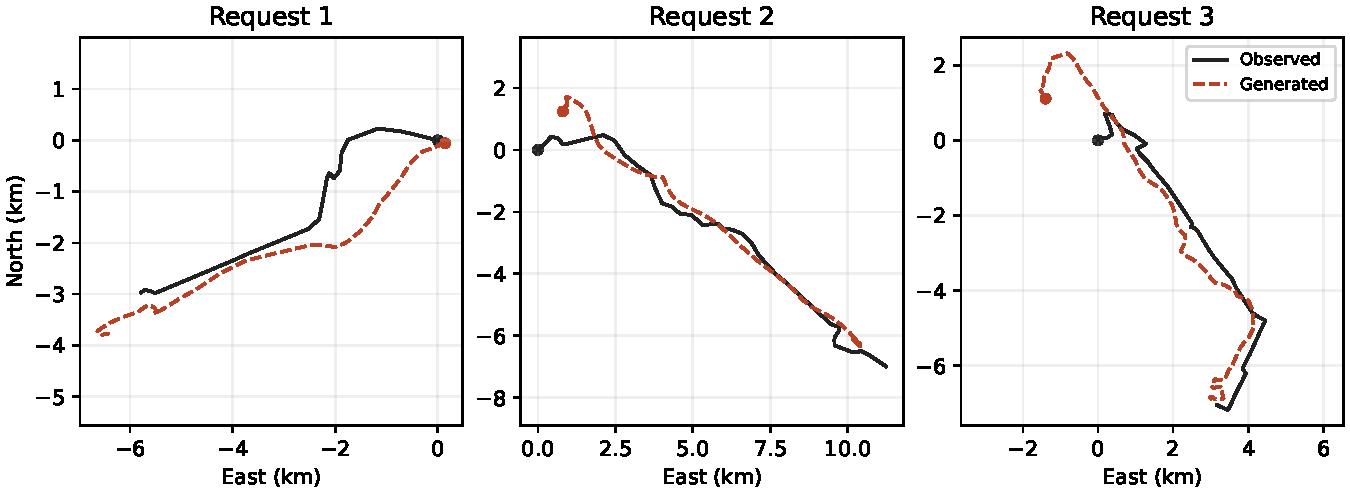
\includegraphics[width=.96\linewidth]{journeys.pdf}\\
\end{center}
\small Figure 1. The first three reserved requests in the fixed evaluation order. Observed and generated positions (batch 56, seed 42) share local axes relative to the observed start. Dots mark departures. Connecting consecutive GPS fixes shows the sampled path at the reporting cadence.

\begin{center}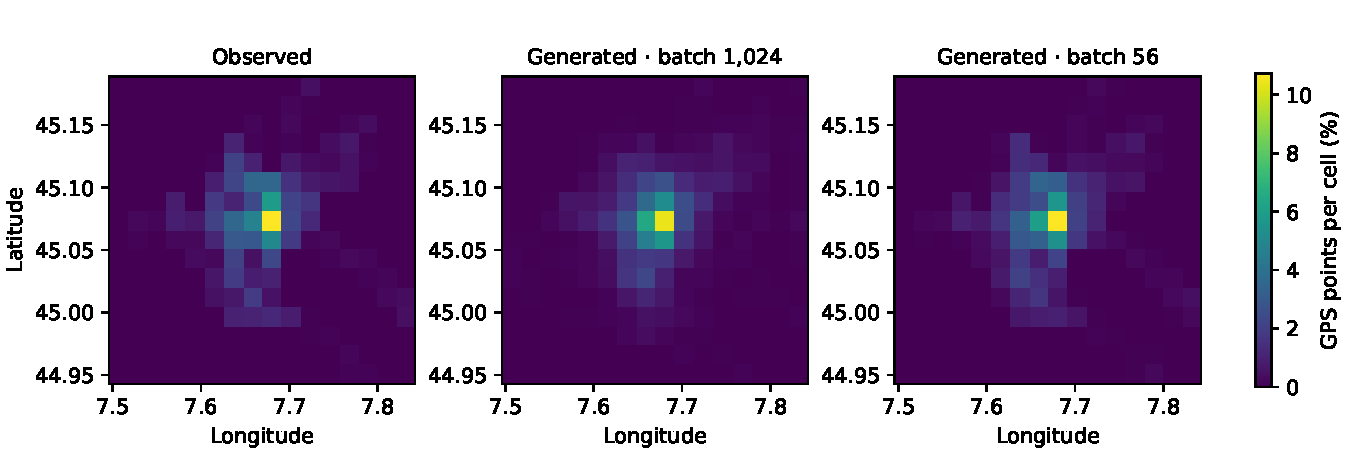
\includegraphics[width=.96\linewidth]{density.pdf}\end{center}
Figure 2. Point occupancy across all 341 requests at seed 42. Each panel uses the same 16 by 16 training grid and colour scale. The full-batch comparison in the table shows why hotspot overlap alone can conceal errors in origin--destination pairs.

\begin{center}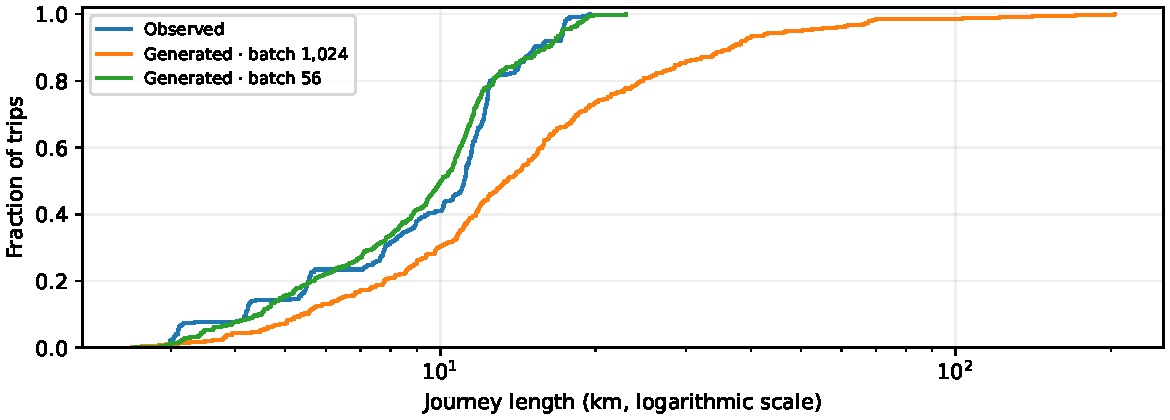
\includegraphics[width=.80\linewidth]{length.pdf}\end{center}
Figure 3. Empirical journey-length distributions for the same requests and seed. The logarithmic distance axis includes the upper tail. At batch 56 the generated median is closer to the observed median.

\end{document}